\documentclass[11pt,aspectratio=169]{beamer}

% ---------------------------------------------------------------------
% Preamble
% ---------------------------------------------------------------------

%--------------------------------------------------------------------
% Pakete
%--------------------------------------------------------------------
\usepackage[T1]{fontenc}       % Korrektes Trennen von Wörtern mit Umlauten
\usepackage[english]{babel}    % Neue deutsche Silbentrennung
\usepackage{hyperref}
\usepackage{graphicx}          % Grafikeinbindung
\usepackage[dvipsnames]{xcolor}
%\usepackage{acro}
\usepackage[withpage]{acronym} % Abkürzungen verwalten
\usepackage{enumitem}          % Listen flexibel anpassen, z.B. keine Einrückung
\usepackage{listings}          % Quellcode einbinden und formatieren
\usepackage[numbers,sort&compress]{natbib} % Zitieren nach [Autor, Jahr] und [1]
\usepackage[zerostyle=d]{newtxtt}
\usepackage{hyphenat}
\usepackage{tikz}
\usepackage{float}
\usepackage{xspace}
\usepackage{lstautogobble}
\usepackage[toc,page]{appendix}
\usepackage[euler]{textgreek} % greek symbols without math environment;
                              % requires texlive-langgreek

\setlength\parindent{0pt}

%\usepackage{epsfig, psfrag}
%\usepackage[multiple]{footmisc}
%
%\usepackage{mdframed}
%
%\usepackage{algorithm}
%%\usepackage{algorithmicx}
%\usepackage{algpseudocode}
%\usepackage{amsmath}
%\usepackage{amssymb}                % Erweiterter Mathematiksatz
%\usepackage{amsthm}
%\usepackage{booktabs}               % Schöne Tabellen mit \toprule\midrule\bottomrule
%\usepackage{calc}                   % Rechnen in LaTeX
%\usepackage[font=small,labelfont=it,format=hang]{caption}[2008/04/01]  %
%\usepackage[right]{eurosym}         % Eurosymbol mit \euro und \EUR{Zahl}
%\usepackage{float}                  % Gleitobjekte fixieren
%\usepackage{footnote}
%\usepackage[left=3cm,right=3cm,top=3cm,bottom=3cm]{geometry}
%%\usepackage[colorlinks=false]{hyperref}             % Links
%\usepackage{hyphenat}               % Umbruch
%\usepackage{ifpdf}
%\usepackage{ifthen}                 % if-Verzeigung
%\usepackage{lmodern}
%\usepackage{multirow}               % Tabellenzelle über mehrere Zeilen
%\usepackage{nomencl}
%\usepackage{paralist}               % Kompakte Listen (Aufzählungen)
%\usepackage{scrpage2}               % KOMA: Kopf- und Fußzeilen ändern
%\usepackage{setspace}
%\usepackage{xspace}
%% Bei Verwendung von lmodern fehlen ein paar Zeichen, z.B. Punkt bei itemize
%% --> Font Warning: Font shape `OMS/lmr/m/n' undefined
%% --> Some font shapes were not available, defaults substituted.
%% Deshalb Paket 'textcomp' laden.
%\usepackage{shortvrb}
%\usepackage{tabularx}               % Tabelle mit fester Gesamtbreite und
%                                    % variabler Spaltenbreite
%\usepackage{textcomp}               % Zusätzliche Sonderzeichen
%%\usepackage[table]{xcolor}          % Erweitertes Farbpaket mit vielen Farbmodellen
%\usepackage{xtab}

%\usepackage[zerostyle=d]{newtxtt}
%\usepackage{tikz}
%\usepackage{float}

\usepackage{fancyvrb}   % BVerbatim

\graphicspath{{./images}}

% ---------------------------------------------------------------------
% Commands
% ---------------------------------------------------------------------

\newcommand{\eg}{\textit{e.g.,}\xspace}
\newcommand{\shortsep}{||}
\newcommand{\sep}{\ ||\ }

\newcommand{\hf}{\ensuremath{H}\xspace}
\newcommand{\pwd}{\mbox{\textit{pwd}}\xspace}
\newcommand{\pw}{\textsc{Catena}\xspace}
%\newcommand{\pwl}{\ensuremath{\textsc{Catena}_{\FL,\hf}}\xspace}
\newcommand{\pwl}{\ensuremath{\textsc{Catena}}\xspace}
%\newcommand{\pwlk}{\ensuremath{\textsc{Catena}^K_{\FL,\hf}}\xspace}
\newcommand{\pwlk}{\ensuremath{\textsc{Catena}^K}\xspace}
\newcommand{\pwbrg}{\textsc{\pw-BRG}\xspace}
\newcommand{\pwdbg}{\textsc{\pw-DBG}\xspace}
\newcommand{\pwhead}{{\large \textsc{Catena}}\xspace}
\newcommand{\pwtitle}{{\LARGE \textsc{Catena}}\xspace}
\newcommand{\pwkg}{\textsc{Catena-KG}\xspace}
\newcommand{\pwax}{\textsc{Catena-Axungia}\xspace}
\newcommand{\pwvar}{\textsc{Catena-Variants}\xspace}
\newcommand{\pwkghead}{{\large \textsc{Catena-KG}}\xspace}

\newcommand{\lmaa}{\pw}
\newcommand{\lmaashort}{\ensuremath{\pw\text{-}\lambda}\xspace}
\newcommand{\lmaatic}{\ensuremath{\pw'\text{-}\lambda}\xspace}
\newcommand{\lamfunc}{\ensuremath{\mbrhfa(\cdot,\cdot)}\xspace}
\newcommand{\FL}{\ensuremath{F}\xspace}
\newcommand{\RL}{\ensuremath{\Gamma}\xspace}
\newcommand{\MHF}{\ensuremath{flap}\xspace}
\newcommand{\seedrand}{\ensuremath{seed\_rand}\xspace}
\newcommand{\updaterand}{\ensuremath{update\_rand}\xspace}


% additional stuff to include pseudocode

%%%%%%%%%%%%%%%%%%%%%%%%%%%%%%%%%%%%%%%%%%%%%%%%%%
% Catena
%%%%%%%%%%%%%%%%%%%%%%%%%%%%%%%%%%%%%%%%%%%%%%%%%%

\newcommand{\catena}{\ensuremath{\mbox{\textsc{Catena-}}\lambda}\xspace}
%\newcommand{\catenabrg}{\textsc{Catena-BRG}\xspace}
%\newcommand{\catenadbg}{\textsc{Catena-DBG}\xspace}
\newcommand{\catenaant}{\textsc{Catena-Dragonfly}\xspace}
\newcommand{\catenaantfull}{\textsc{Catena-Dragonfly-Full}\xspace}
\newcommand{\catenabut}{\textsc{Catena-Butterfly}\xspace}
\newcommand{\catenabutfull}{\textsc{Catena-Butterfly-Full}\xspace}
\newcommand{\catenawl}{\textsc{Catena}\xspace}
\newcommand{\catenakg}{\ensuremath{\mbox{\texttt{Catena-KG}}}\xspace}
\newcommand{\lbrg}{\ensuremath{\lambda\mbox{\texttt{-BRG}}}\xspace}
\newcommand{\lbrh}{\ensuremath{\lambda\mbox{\texttt{-BRH}}}\xspace}

\newcommand{\romix}{\texttt{ROMix}\xspace}
\newcommand{\romixmc}{\texttt{ROMixMC}\xspace}
\newcommand{\scrypt}{\texttt{scrypt}\xspace}

\newcommand{\header}{\ensuremath{H}\xspace}
\newcommand{\Garlic}{\ensuremath{G}\xspace}
\newcommand{\garlic}{\ensuremath{g}\xspace}
\newcommand{\inp}{\ensuremath{x}\xspace}
\newcommand{\salt}{\ensuremath{s}\xspace}
\newcommand{\tweak}{\ensuremath{U}\xspace}
\newcommand{\node}[1]{\ensuremath{v_{#1}}\xspace}
\newcommand{\nodes}{\ensuremath{\mathfrak{V}}\xspace}
\newcommand{\graph}{\ensuremath{\Pi(\nodes,\edges)}\xspace}
\newcommand{\ggraph}{\ensuremath{\Pi_\garlic^\lambda(\nodes,\edges)}\xspace}

\renewcommand{\H}{\ensuremath{\mathcal{H}}\xspace}
\renewcommand{\algorithmicrequire}{\textbf{Input:}}
\renewcommand{\algorithmicensure}{\textbf{Output:}}

\newcommand{\mbrgfax}{\ensuremath{\lambda\text{-BRG}}\xspace}
\newcommand{\mbrhfax}{\ensuremath{\lambda\text{-BRH}}\xspace}
\newcommand{\mbrhfaxm}{\ensuremath{\lambda\text{-}BRH}\xspace}
\newcommand{\mbrhfa}{\ensuremath{BRH_\lambda^g}\xspace}


\newcommand{\testentry}[3]{\textbf{#1} & \texttt{#2} & (#3 octets)\\}

\newcommand{\blake}{BLAKE2b\xspace}
\newcommand{\blakefast}{BLAKE2b-1\xspace}

\newcommand{\length}[1]{\ensuremath{|#1|}\xspace}

\newcommand{\glow}{\ensuremath{\garlic_{\text{low}}}\xspace}
\newcommand{\ghigh}{\ensuremath{\garlic_{\text{high}}}\xspace}


\newcommand{\catenabrg}{\textsc{Catena-BRG}\xspace}
\newcommand{\catenadbg}{\textsc{Catena-DBG}\xspace}
\newcommand{\hfinit}{\ensuremath{H_{\text{init}}}\xspace}
\newcommand{\hffirst}{\ensuremath{H_{\text{first}}}\xspace}

\newcommand{\overviewPDF}{\includegraphics[height=0.85\textheight]{Overview.eps}}


%%%%%%%%%%%%%%%%%%%%%%%%%%%%%%%%%%%%%%%%%%%%%%%%%%
% pseudo code

\newcommand{\pscatena}{\
    \begin{algorithm}[H] \caption*{\pw}
      \begin{algorithmic}[1]
        \REQUIRE $pwd$, $t$, $s$, \glow, \ghigh, $m$, $\gamma$
        \ENSURE $x$
        \STATE $x \gets \hf(t \sep pwd \sep s)$
        \STATE $x \gets \MHF(\lceil \glow/2\rceil,x,\gamma)$
        \label{line:mhf}
        \FOR{$g=\glow,\ldots,\ghigh$}
          \STATE $x \gets \MHF(g,x \sep 0^*,\gamma)$
          \label{line:tabula-catena}
          \STATE $x \gets \hf(g \sep x)$
          \STATE $x \gets truncate(x,m)$
        \ENDFOR
        \RETURN $x$
      \end{algorithmic}
      \label{alg:catena}
    \end{algorithm}}

\newcommand{\psflap}{\
    \begin{algorithm}[H]
    \caption*{\MHF}
      \begin{algorithmic}[1]
        \REQUIRE $g$, $x$, $\gamma$
        \ENSURE $x$
        \STATE $(v_{-2},v_{-1}) \gets \hfinit(x)$
        \label{line:init1}
        \FOR{$i=0 ,\ldots, 2^g-1$}
        \label{line:loop1-1}
          \STATE $v_i \gets H'(v_{i-1}\sep v_{i-2})$
          \label{line:loop1-2}
        \ENDFOR
        \label{line:init2}
        \STATE $v \gets \RL(g,v,\gamma)$
        \label{line:public_input}
        \STATE $x \gets \FL(v)$
        \label{line:memory_hard}
        \STATE \textbf{return} $x$
      \end{algorithmic}
      \label{alg:mhf}
    \end{algorithm}}

\newcommand{\pshinit}{\
    \begin{algorithm}[H]
    \caption*{\hfinit}
      \begin{algorithmic}[1]
        \REQUIRE $x$
        \ENSURE $v_{-2},v_{-1}$
        \STATE $\ell = 2\cdot k/n$
        \FOR{$i=0,\ldots,\ell-1$}
        \label{line:init-large-1}
          \STATE $w_i \gets \hf(i\sep x)$
          \label{line:hfinit-hf}
        \ENDFOR
        \STATE $v_{-2} \gets (w_0\sep\ldots\sep\ w_{\ell/2-1})$
        \STATE $v_{-1} \gets (w_{\ell/2}\sep\ldots\sep\ w_{\ell-1})$
        \STATE \textbf{return} $(v_{-2},v_{-1})$
        \label{line:init-large-2}
      \end{algorithmic}
      \label{alg:hfinit}
    \end{algorithm}}

\newcommand{\psciupdate}{\
    \begin{algorithm}[H]
    \caption*{Client-Independent Update}
      \begin{algorithmic}[1]
        \REQUIRE $h, g_{high}, \lambda, m, \gamma, {g'}_{high}$
        \ENSURE $h'$
        \STATE $h' \gets h$
        \FOR{$g=g_{high},\ldots,{g'}_{high}$}
          \STATE $h' \gets flap(g,h' \sep 0^*,\gamma,\lambda)$
          \STATE $h' \gets H(g\sep h')$
          \STATE $h' \gets truncate(h',m)$
        \ENDFOR
        \STATE \textbf{return} $h'$
      \end{algorithmic}
    \end{algorithm}}

\newcommand{\pskg}{\
    \begin{algorithm}[H]
    \caption*{\pw-KG}
      \begin{algorithmic}[1]
        \REQUIRE $pwd, t', s, g_{low}, g_{high}, \gamma, \ell, \mathcal{I},
        \lambda$
        \ENSURE $k$
        \STATE $x \gets \pw(pwd, t', s, g_{low}, g_{high}, n, \gamma)$
        \STATE $k \gets \emptyset$
        \FOR{$i=1,\ldots,\lceil\ell/m\rceil$}
          \STATE $k \gets k \sep H(i \sep \mathcal{I} \sep \ell \sep x)$
        \ENDFOR
        \STATE \textbf{return} $(k, \ell)$
      \end{algorithmic}
    \end{algorithm}}

\usepackage{color}
\definecolor{gray}{rgb}{0.4,0.4,0.4}
\definecolor{darkblue}{rgb}{0.0,0.0,0.6}
\definecolor{cyan}{rgb}{0.0,0.6,0.6}

\lstset{
  basicstyle=\ttfamily,
  columns=fullflexible,
  showstringspaces=false,
  commentstyle=\color{gray}\upshape
}

\lstdefinelanguage{XML}
{
  morestring=[b]",
  morestring=[s]{>}{<},
  morecomment=[s]{<?}{?>},
  stringstyle=\color{black},
  identifierstyle=\color{darkblue},
  keywordstyle=\color{cyan},
  morekeywords={xmlns,version,type}% list your attributes here
}

\usetheme{CambridgeUS}


\definecolor{midnightblue}{rgb}{0,.25,.5}
\definecolor{darkblue}{rgb} {0.125,0.25, 0.625}
\definecolor{darkgreen}{rgb}{0.125,0.625,0.25}
%\definecolor{darkred}{rgb}  {0.625,0.125,0.25}
\definecolor{darkred}{rgb}  {0.0,0.4,0.59}

\mode<presentation>
{
  \useinnertheme{rectangles}
  \setbeamertemplate{navigation symbols}{}
}

\setbeamercolor{footlinecolorl}{fg=black,bg=lightgray}
\setbeamercolor{footlinecolor}{fg=black,bg=gray}
\setbeamercolor{footlinecolord}{fg=black,bg=darkgray}
\setbeamercolor{block title}{bg=darkred,fg=white}

\setbeamertemplate{itemize item}{\color{darkred}$\blacksquare$}
\setbeamertemplate{itemize subitem}{\color{darkred}$\blacktriangleright$}
\setbeamercolor{item projected}{bg=darkred}
\setbeamertemplate{enumerate items}[default]
\setbeamercolor{enumerate item}{fg=darkred}
\setbeamercolor{enumerate subitem}{fg=darkred}
\setbeamercolor{enumerate subsubitem}{fg=darkred}

\setbeamertemplate{footline}{%
\hbox{%
\begin{beamercolorbox}[wd=.40\paperwidth,ht=4.25ex,left,leftskip=3ex]{author in head/foot}%
    \vbox to4.25ex{\vfil\hbox{\usebeamerfont{author in head/foot} \insertshortauthor}\vfil}%
\end{beamercolorbox}%
\begin{beamercolorbox}[wd=.25\paperwidth,ht=4.25ex,center]{title in head/foot}%
    \vbox to4.25ex{\vfil\hbox{\usebeamerfont{date in
    head/foot}\insertshorttitle{}}\vfil}%
\end{beamercolorbox}%
\begin{beamercolorbox}[wd=.05\paperwidth,ht=4.25ex,center]{title in head/foot}%
    \vbox to4.25ex{\vfil\hbox{\usebeamerfont{title in head/foot}\insertframenumber/\inserttotalframenumber}\vfil}%
\end{beamercolorbox}%
\begin{beamercolorbox}[wd=.30\paperwidth,ht=4.25ex,right,rightskip=3ex]{date in head/foot}%
    \vbox to4.25ex{\vfil\hbox{\insertshortdate{}}\vfil}%
\end{beamercolorbox}}%
}

%\setbeamertemplate{footline}{
%  \quad \tiny \insertshortauthor \hfill \insertshorttitle \qquad \hfill \insertshortdate\ \qquad\qquad
%}


% ---------------------------------------------------------------------
% Title
% ---------------------------------------------------------------------

\title[Green Development]{Supporting the Discovery of Energy Hot-Spots via Performance Alignment}
%\subtitle{Subtitle (project name)}
\author[M. Weber]{Max Weber}
\institute[Bauhaus-Universität Weimar]{}
\date[\today]{\today}

\raggedright
\AtBeginSection{\frame{\sectionpage}}

% ---------------------------------------------------------------------

\begin{document}

% ---------------------------------------------------------------------
% Content
% ---------------------------------------------------------------------

\maketitle

%\begin{frame}{Outline}
%\tableofcontents
%\end{frame}

% ---------------------------------------------------------------------
%\section{Subject of this Thesis}
% ---------------------------------------------------------------------

\begin{frame}{Subject of this Thesis}
  \begin{itemize}
    \item support developers as early as possible by finding energy hotspots in their source code
    \item enables:
    \begin{itemize}
      \item reduction of overall energy consumption for future software
      \item detection of possible energy hotspots in existing software
    \end{itemize}
  \end{itemize}
\end{frame}

% ---------------------------------------------------------------------
%\section{Overview/Process/Progress/Current State}
% ---------------------------------------------------------------------

\begin{frame}{Overview}
  \begin{center}
    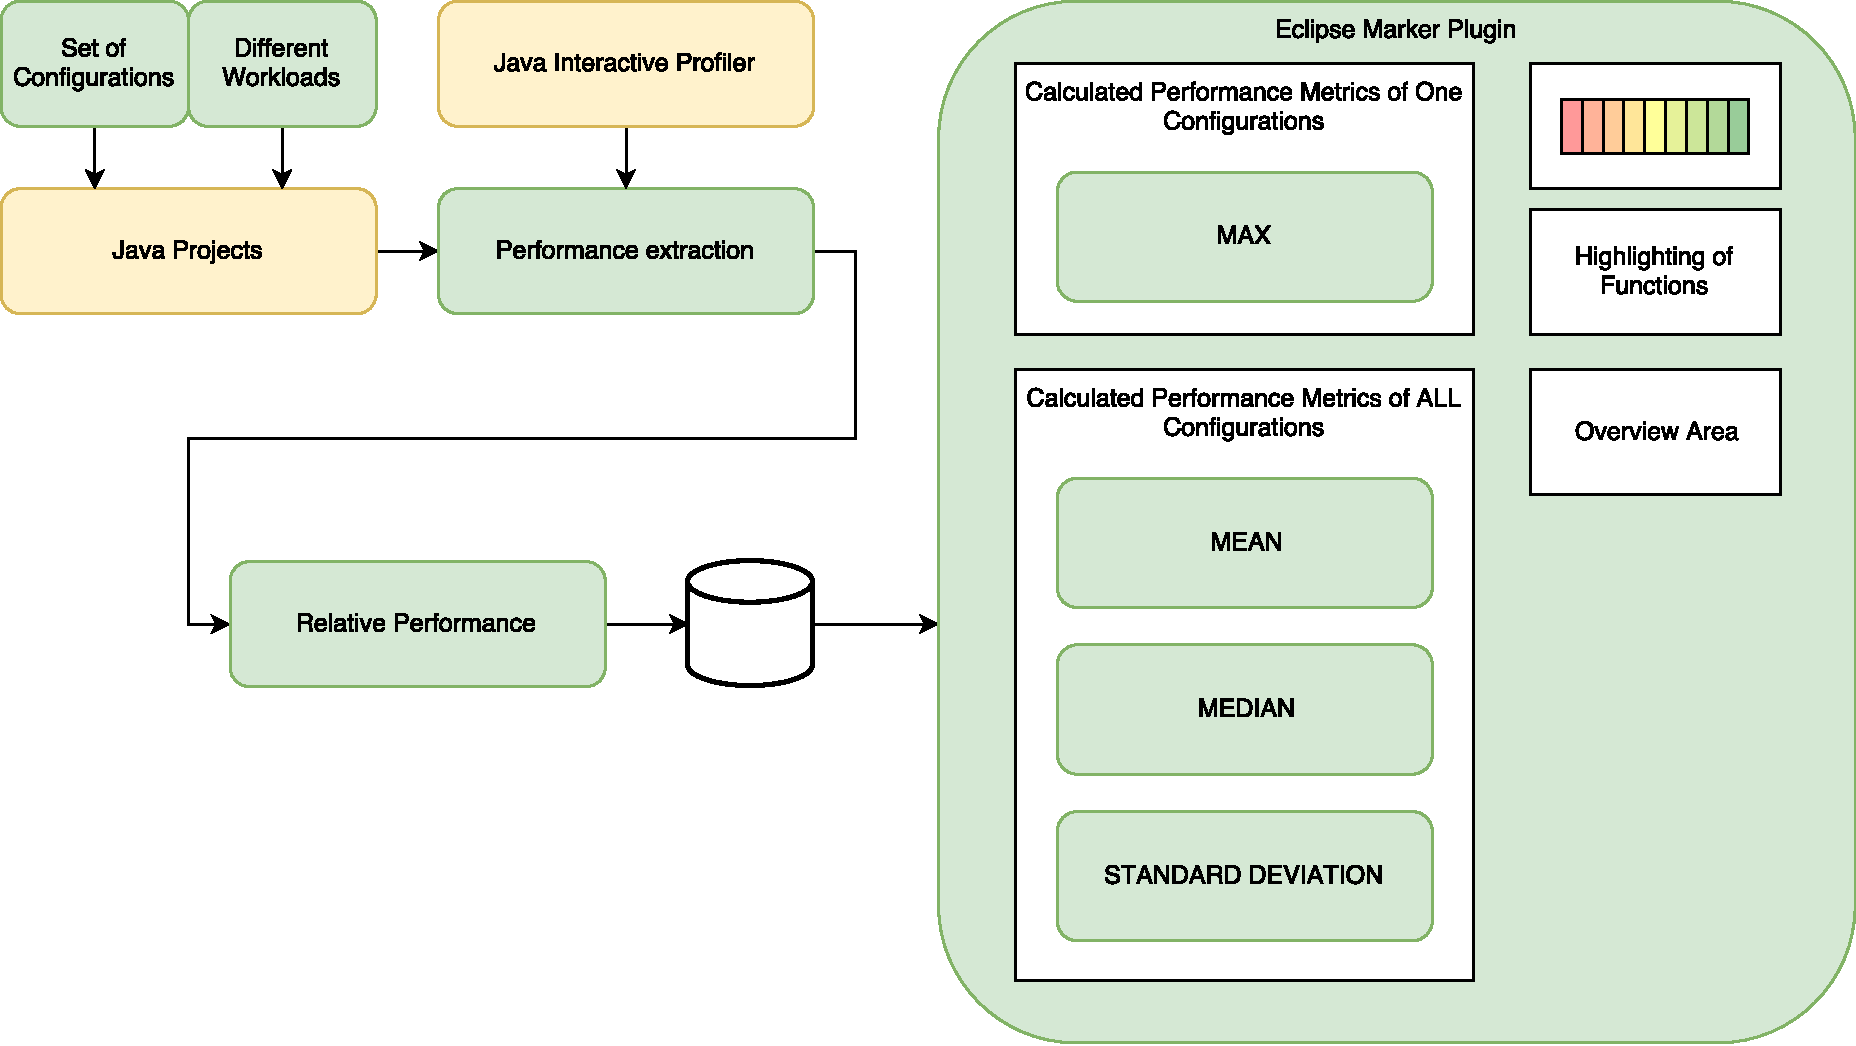
\includegraphics[height=0.83\textheight]{./images/Workflow_Green_DEV_0.pdf}
  \end{center}
\end{frame}

% ---------------------------------------------------------------------
%\section{Projects}
% ---------------------------------------------------------------------

\begin{frame}{Data Sets}
  \begin{itemize}
    \item requirements:
    \begin{itemize}
      \item analyzable
      \item configurable
      \item scalable (workload)
    \end{itemize}
    \item restriction to Java projects because: widespread, popular, many different projects to choose from
  \end{itemize}
\end{frame}

\begin{frame}{Catena - Password Hashing}
  \begin{itemize}
    \item password hashing framework
    \item use of BLAKE2b as a fast and secure cryptographic hash function
    \item developed at Bauhaus Universität Weimar (Chair of Media Security)
    \pause
    \item available in Java, Rust, Python, C++, JavaScript
    \item heavily tested over all implementations
    \item configuartion space: 3,565,158,400
    \item workload is length of password to be hashed
  \end{itemize}
\end{frame}

\begin{frame}{H2 - Database}
  \begin{itemize}
    \item SQL database
    \item pure Java
    \item open-source
    \item configuration space: 65,536,000
    \item workload is number of database entries to perform queries on
  \end{itemize}
\end{frame}

\begin{frame}{Sunflow - Ray Tracing}
  \begin{itemize}
    \item image generation through ray tracing
    \item pure Java
    \item open-source
    \item one default scene
    \item configuration space: 6,400,000
    \item workload is size of images to be generated (64x64, 128x128, 256x256)
  \end{itemize}
\end{frame}

% ---------------------------------------------------------------------
%\section{Performance Extraction}
% ---------------------------------------------------------------------

\begin{frame}{JIP - Java Interactive Profiler}
  \begin{itemize}
    \item pure Java
    \item open source
    \item light-weight
    \item measures net time: removes overhead of gathering performance data
    \item wraps each method with profiling code
  \end{itemize}
\end{frame}

\begin{frame}{Profiling}
  \begin{itemize}
    \item 400 different configurations
    \item 3 different workloads
    \item n times to average performance (reduce external measurement impact)
  \end{itemize}
\end{frame}

% ---------------------------------------------------------------------
%\section{Relative Performance}
% ---------------------------------------------------------------------

\begin{frame}{Relative Execution Time per Function}
  \begin{itemize}
    \item profiler output per configuration and workload
    \item $performance(a) = (time(a)/calls_a)*100/(time(x)/calls_x)$
    \item $x$ = execution time of function with highest execution time per sample
    \item $a$ = execution time of current function
  \end{itemize}
\end{frame}

% ---------------------------------------------------------------------
%\section{Eclipse Marker Plugin}
% ---------------------------------------------------------------------

\begin{frame}{Plugin - Current State}
  \begin{center}
    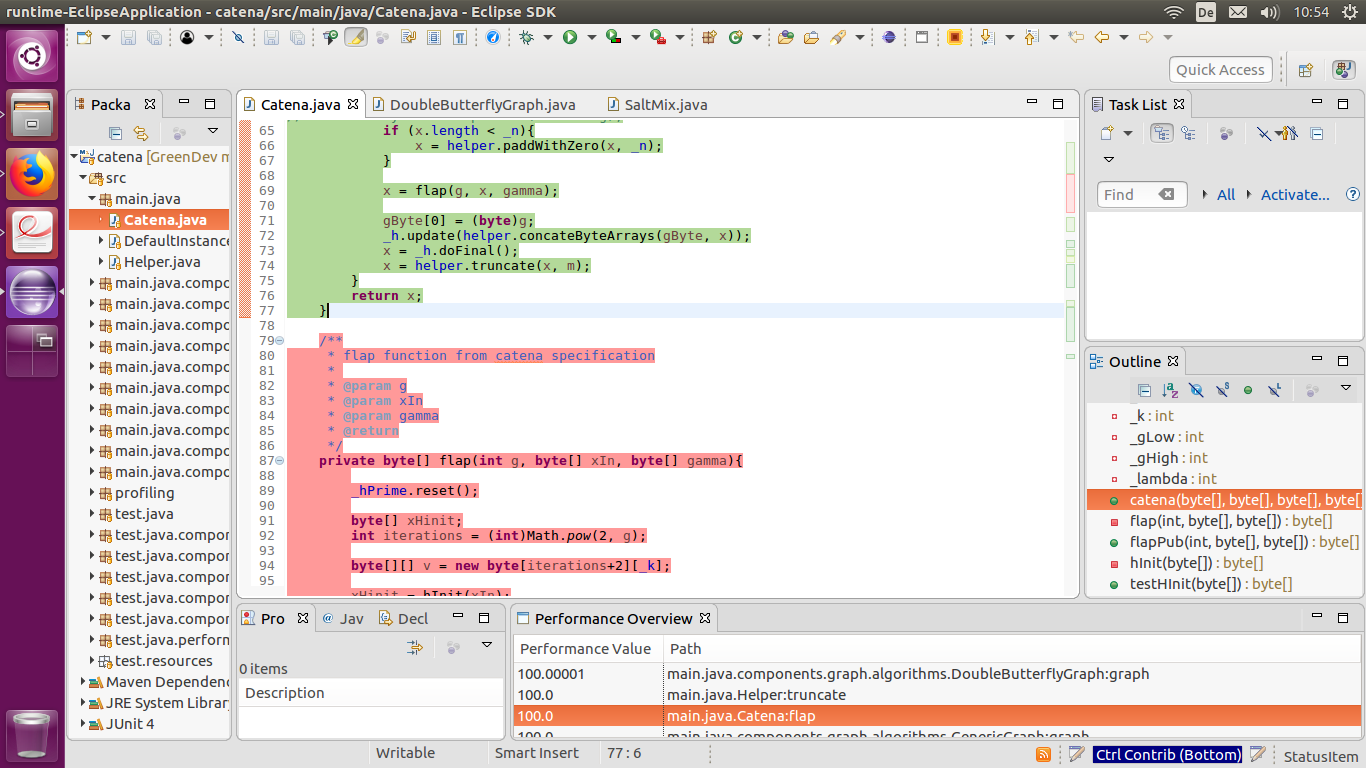
\includegraphics[height=0.83\textheight]{./images/catena_max_all_cfgs}
  \end{center}
\end{frame}

% ---------------------------------------------------------------------
%\section{Next Steps}
% ---------------------------------------------------------------------

\begin{frame}{ToDo - Predict Performance}
  \begin{itemize}
    \item performance of unknown configurations
    \item allow user to input config of interest
    \item predict performance of function:
    \begin{itemize}
      \item single-objective optimization
      \item multi-objective optimization (sunflow: performance, image quality)
      \item perceptron learning      
    \end{itemize}
  \end{itemize}
\end{frame}

\begin{frame}{ToDo - Align Performance and Energy Consumption}
  \begin{itemize}
    \item correlation between performance and energy consumption 
    \item for each project and each configuration
    \item (Pearson Correlation Coefficient?)
    \item (SPL conqueror?)
  \end{itemize}
\end{frame}

\begin{frame}{Questions}
  \begin{itemize}
    \item influence of test environment on performance measurement (hardware, os, ...)
    \item configuration sampling strategy
    \item correlation of performance and energy consumption
  \end{itemize}
\end{frame}

%\section{Appendix}

\begin{frame}{Catena Configuration Space}
  \begin{itemize}
    \item (2) HASH
    \item (2) GAMMA
    \item (4) GRAPH
    \item (2) PHI

    \item (17) $g_{low}=g_{high}$: garlic
    \item (100) $\lambda$: lambda
    \item (256) $v\_id$: version id
    \item (256) $d$: mode of Catena
  
    \item (byte[]) $\gamma$: gamma (only required if GAMMA)
    \item (byte[]) $AD$: optional associated data
    \item (byte[]) $V$: unique version identifier (defined by default)
  \end{itemize}
  Overall configuration space: 3,565,158,400
\end{frame}

\begin{frame}{H2 Configuration Space}
  \begin{itemize}
    \item (40) ANALYZE AUTO
    \item (100) ANALYZE SAMPLE
    \item (2)*14 COMPRESS, EARLY FILTER, MULTI THREADED, MV STORE, OPTIMIZE EVALUATABLE SUBQUERIES, OPTIMIZE IN LIST, OPTIMIZE IN SELECT, OPTIMIZE INSERT FROM SELECT, OPTIMIZE IS NULL, OPTIMIZE OR, OPTIMIZE TWO EQUALS, PAGE STORE INTERNAL COUNT, RECOMPILE ALWAYS, ROWID
  \end{itemize}
  Overall configuration space: 65,536,000
\end{frame}

\begin{frame}{Sunflow Configuration Space}
  \begin{itemize}
    \item (10) threads
    \item (10) diffuseDepth
    \item (10) reflectionDepth
    \item (10) refractionDepth
    \item (54) bucketSize
    \item (10) samples
  \end{itemize}
  Overall configuration space: 6,400,000
\end{frame}
%-----------------------------------------------------------------------
% Appendix
% ---------------------------------------------------------------------

\appendix
\end{document}
